\documentclass[a4paper,12pt]{article} %style de document
\usepackage[utf8x]{inputenc} %encodage des caractères
\usepackage[french]{babel} %paquet de langue français
\frenchbsetup{StandardLists=true}
\usepackage[T1]{fontenc} %encodage de la police
\usepackage{geometry}
\geometry{left=1cm, right=1cm, top=2cm, bottom=2cm} %marges
\usepackage{graphicx} %affichage des images
\usepackage{enumitem}
\usepackage{amssymb}
\usepackage{hyperref}
\usepackage{verbatim}
\usepackage{setspace}
\usepackage{tabto}
\usepackage[hypcap=false]{caption}
\usepackage{subcaption}

\usepackage{fancyhdr}
\usepackage{fancybox}
\setlength{\headheight}{14.61858pt}
\addtolength{\topmargin}{-0.11859pt}
\pagestyle{fancy}
\lfoot{}
\cfoot{}
\rfoot{\bf page \thepage}
\lhead{\rightmark}
\chead{}
\rhead{\leftmark}
\newcommand{\Touche}[1]{\Ovalbox{#1}}
\renewcommand{\headrulewidth}{0pt}
\renewcommand{\footrulewidth}{1pt}

\author{
	\textbf{LEDOUX Eloi},\\
	\textbf{TAUPIN Erwann},\\
	\textbf{KITSOUKOU Manne Emile},\\
	\emph{L1 informatique},\\
	\emph{Groupe 2B},\\
	\textsc{Projet SOKOBAN}\\}
   
\date{Avril 2021}

\title{
	\rule{0.75\textwidth}{2pt}\\
	\textbf{CONCEPTION LOGICIEL :\\ RAPPORT DE DÉVELOPPEMENT DU PROJET} 
	\rule{0.75\textwidth}{2pt}\\}

\begin{document} %début du document
\maketitle
\begin{center}

\includegraphics[scale=1]{images/LogoUNICAEN.png}\\
\end{center}
\thispagestyle{empty}
\newpage

\renewcommand{\contentsname}{Sommaire}
\tableofcontents
\thispagestyle{empty}
\newpage

\section{Introduction}
\setcounter{page}{1}
\onehalfspacing

\subsection{Choix du sujet}
Suite à la création du groupe nous devions choisir un sujet parmi ceux proposés. Nous nous sommes rapidement entendus sur la réalisation d'un Sokoban.
 
Le Sokoban est un jeu vidéo dans lequel le joueur doit ranger des caisses sur des cases prédéfinies. Pour cela, le joueur peut se déplacer dans les quatre directions, mais il ne peut pousser qu'une seule caisse à la fois, de plus, il n'a pas la possibilité de la tirer.

Une fois que toutes les caisses sont sur les cases cibles, le joueur passe au niveau suivant. L'objectif du jeu est de réussir à compléter les différents niveaux avec le moins de coups possibles.

\subsection{Les objectifs du projet}

Dès le départ, nous avions plusieurs objectifs principaux que nous voulions réussir à mettre en place, mais aussi quelques objectifs secondaires que nous souhaitions implémenter s'il nous restait suffisamment de temps.

Au début du projet, nous avions trois objectifs principaux. Le premier était d'avoir un jeu jouable et plutôt joli. Le second était assez simple mais nous a demandé un peu de réflexion : nous souhaitions avoir la possibilité d'importer de nouveaux niveaux en les déposant simplement dans un répertoire spécifique. Et enfin, le troisième objectif était de laisser la possibilité au joueur de choisir le niveau sur lequel il souhaite commencer, et de pouvoir à tout moment revenir au menu principal et sélectionner un autre niveau.

Au fur et à mesure de l'avancement du projet, certains objectifs secondaires sont devenus des objectifs principaux, par exemple, la possibilité de revenir d'un ou plusieurs coups en arrière, la possibilité de réinitialiser un niveau, ou encore l'ajout d'un score.

Lorsque l'on a constaté que le projet avançait assez rapidement et sans trop de difficultés, nous avons décidé d'ajouter d'autres fonctionnalités. Parmi celles-ci, on peut citer l'ajout d'un écran de fin indiquant le score lorsque tous les niveaux sont complétés, mais aussi l'ajout de son (au début d'un niveau, mais aussi à chaque coup). Une fois le son ajouté, une autre fonctionnalité s'est imposée : la possibilité de couper le son !

Enfin, une fois les fonctionnalités précédentes ajoutées, nous avons voulu implémenter un solveur / un algorithme de résolution, qui permet de résoudre les niveaux automatiquement.

\section{Travaux préliminaires}

\subsection{Renseignement sur le Sokoban} 

Avant de nous lancer dans la création de fonctions et l'écriture du code, nous avons cherché des renseignements sur le Sokoban, son fonctionnement, ainsi que sur le format sok. La page \href{https://fr.wikipedia.org/wiki/Sokoban}{Wikipedia du Sokoban} nous a bien aidé à comprendre le fonctionnement de ce jeu, et le site \href{http://sokobano.de/wiki/index.php?title=Sok_format}{sokobano.de} nous en a appris plus sur le format sok utilisé pour les fichiers des différents niveaux.

\subsection{Répartition des fichiers}

Une fois les recherches préliminaires effectuées, nous avons pu réfléchir à la façon dont nous allions répartir les différentes fonctions.
\\
Nous voulions, au départ, avoir trois fichiers :
\begin{itemize}
	\item un fichier Grille, regroupant les fonctions de base permettant de modifier une grille;
	\item un fichier Level, qui hériterait de Grille, et qui appliquerait les fonctions de base à notre jeu;
	\item enfin, un fichier Gestion, qui pourrait gérer intégralement une partie de Sokoban.
\end{itemize}

Cependant, au fur et à mesure que nous avancions, nous nous sommes aperçus que nous ne pourrions pas garder cette répartition.
\\
Ainsi, nous avons désormais six fichiers :
\begin{itemize}
	\item un fichier grille \ref{Grille}, qui regroupe les fonctions de base permettant de modifier une grille;
	\item un fichier level \ref{Level}, qui hérite de Grille, et qui applique les fonctions de base à notre jeu;
	\item un fichier multimedia \ref{multimedia}, qui permet de gérer les images ainsi que le son;
	\item un fichier solver, qui contient le code du solveur que nous avons récupéré et dont nous nous servons;
	\item un fichier frame \ref{couche}, qui contient les différents écrans de jeu;
	\item enfin, un fichier main, qui permet de gérer la partie de Sokoban.
\end{itemize}

\subsection{La répartition des tâches}

Dès le début, il a été clair que la réalisation du projet serait réalisée de la façon la plus collective possible. Ainsi, pour une meilleure efficacité, nous avons décidé que chacun devrait toucher en partie à l'ensemble des implémentations qui auront été effectuées.
C'est ainsi que:
\begin{itemize}
	\item Eloi et Emile se sont chargés du développement du module grille
	\item Le module Level a été développé par Erwann avec la collaboration de Eloi et Emile pour le développement des déplacements dans un niveau
	\item Erwann, en collaboration avec Eloi, s'est occupé principalement du module frame
	\item Erwann s'est occupé de la recherche d'un algorithme fonctionnel pour l'IA
	\item Emile s'est chargé du module multimédia
	\item L'intégration de l'algorithme a été pensée par l'ensemble du groupe 
	\item L'ensemble du rapport et du diaporama a été réalisé collectivement
\end{itemize}
Cette répartition reflète uniquement de façon exhaustive les acteurs lors de l'implémentation de chaque partie. Mais dans le fond, il faut souligner la dévotion et l'engagement de chacun
dans le développement du projet. Car, tous les membres du groupes ont apporté leur collaboration autant pour comprendre la tâche des autres mais aussi pour parfaire les idées de chacun.

\section{Structure du projet}

\subsection{Fichier de structure d'une grille}

Lors de nos premières réflexions sur le projet, l'idée qui nous a été confiée par nos enseignants fût d'envisager le jeu de Sokoban comme un jeu entièrement jouable au travers de tableaux Python en deux dimensions. Pour cela, il nous fallait donc trouver un moyen de gérer, en simultané, le jeu à travers la grille, la lecture du niveau, ainsi que les actions du joueur. Notre réponse à cette problématique a alors été d'envisager ces paramètres à travers deux classes: une classe Grille regroupant le plus de possibilités d'interactions envisageables avec un tableau en deux dimensions, sans lien réel avec le Sokoban, et une classe Level héritant de Grille qui adapterait un niveau de Sokoban en tableau et permettrait de gérer ce même tableau au travers de fonctions plus spécifiques au jeu lui même.

\subsubsection{Création d'un fichier de grille global}

L'un de nos premiers objectifs lors de notre passage sur machine fût donc de concevoir un fichier Python de manipulation de listes en plusieurs dimensions. Ce fichier devait être suffisamment exhaustif pour proposer l'intégralité des opérations qui nous serait nécessaire par la suite lors de la création du jeu, mais devait être aussi réutilisable dans l'éventualité où nous souhaiterions créer un autre jeu/une autre application nécessitant des manœuvres sur grilles. 
\\
Tout d'abord, nous avons commencé par regrouper les fonctions "basiques" de manipulation de listes que nous connaissions dans une classe intitulée "Grille". Dans un souci d’exhaustivité, bien que nous ayons essayé de créer un maximum de fonctions par nous même, nous avons fini par le compléter en y ajoutant des fonctions reprises du cours de programmation du premier semestre.
\\
Ainsi, la classe Grille devient le cœur de notre projet, où plutôt son squelette. Son fonctionnement est assez basique: la classe prend en paramètre un nombre de lignes et un nombre de colonnes puis utilise des paramètres lors de son initialisation pour créer un tableau vide aux dimensions convenues, récupérable sous le nom de "plateau". Ce plateau a pour intérêt de pouvoir : apporter des modifications à la grille, l'afficher d'une certaine façon en console, ou encore vérifier la présence/l'emplacement de certains éléments dans le tableau à partir des fonctions de la classe Grille. L'idée est ici de pouvoir mettre en place une classe qui pourra servir à une future classe, celle-ci nous permettra de transformer un fichier de niveau de jeu en une grille de plateau.
\\
Le lot de fonctions le plus utile à ce stade du développement regroupe toutes les fonctions permettant de traiter des données du tableau à travers leur numéro de cellule. En pratique, pour chaque colonne de chaque ligne du tableau, la fonction \texttt{trouve case} associe un numéro de case qu'il sera possible de retrouver/modifier avec les fonctions de la classe. Cet ajout est particulièrement utile pour retrouver l'emplacement d'un certain symbole au sein du plateau créé/modifié par la fonction mais se révélera encore plus efficace lorsqu'il s'agira de reconnaître les différents éléments qui composent un niveau de Sokoban.
\newpage
Enfin, dans cette optique de "préparation", nous avons amorcé la représentation graphique du jeu en appliquant en paramètre de la classe Grille la possibilité de choisir la taille d'une case du tableau, en pixel, ainsi que la marge qui l'accompagne, l'idée étant de se préparer à toute éventualité. Au moment de la création de la classe ce concept demeurait cependant relativement abstrait, en effet, aucun d'entre nous n'avait auparavant travaillé avec Pygame ou une quelconque interface graphique. 

\subsubsection{Lecture d'un niveau de Sokoban}

Comme dit précédemment, une fois la classe Grille fonctionnelle, il était ensuite nécessaire de la faire hériter par une autre classe de gestion de tableaux possédant une initialisation et des fonctions plus spécifiques au jeu du Sokoban. C'est dans cette optique que nous avons conçu la classe Level.
\\
Pour parfaitement comprendre cette classe, il est important de comprendre son fonctionnement. A l'instar de la classe Grille, la classe Level va construire un tableau qui, cette fois, ne sera pas vide mais contiendra l’intégralité des symboles qui composent le niveau de Sokoban (en .sok) désiré. Pour se faire, la classe prend en paramètre un chemin vers le niveau de Sokoban puis à l'initialisation, la classe va lire ce niveau en le stockant dans une variable.
\\
La construction du niveau s'opère ensuite grâce à la formation particulière d'un niveau de Sokoban. Il faut savoir qu'un fichier .sok comprenant un tel niveau s'organise comme un fichier texte dont la première ligne contient les données du nombre de colonnes et des lignes (dans cet ordre) du niveau en question. Ainsi, la classe peut alors récupérer ces données afin de les utiliser pour initialiser un tableau vide aux bonnes dimensions à partir de la fonction Grille. Ensuite, cette même grille sera remplie ligne par ligne à partir de la deuxième ligne du fichier où débute la représentation du niveau (voir annexe A). Pour ce faire, on utilise une boucle comme suit :
\\
\textbf{\emph{
\tabto{2em}pour ligne de fichier[2e ligne] \\
	\tabto{4em}plateau[ligne] = liste(replace plateau[ligne] par fichier[ligne])
}}
\\
Ainsi, on obtient un tableau en deux dimensions aux proportions désirés contenant pour chaque case un symbole de la représentation du niveau. De ce fait, on peut à partir de ce moment là, considérer que l'on a obtenu une représentation du niveau manipulable par les fonctions de la classe Grille ainsi que par de futures fonctions de jeu.
\\
Il est important de noter aussi qu'une fois ce travail effectué, la classe sauvegardera l'état initial du niveau dans une variable nommée "historique". Un ajout qui nous permettra, plus tard, de gérer une fonction de "reset" du niveau.

\subsubsection{Adaptation des symboles pour le programme}
 
Une fois le niveau adapté sous forme de plateau de jeu à travers un tableau Python en deux dimensions, il nous était désormais possible d'y apporter des modifications à l'aide de fonctions de la classe Grille. Si nous avions déjà envisagé comment gérer les déplacements du personnage lors de nos travaux préliminaires, il fallait d'abord trouver un moyen de communiquer à la machine comment identifier ce même personnage au sein de la grille ainsi que tous les obstacles qui pourraient être rencontrés par ledit personnage.
\newline
Dans un premier temps, voici une liste des différents symboles qui composent un niveau de Sokoban et qui, par conséquent, devront être explicités à la machine afin de leur attribuer différents comportements:
\begin{itemize}
\item \texttt{@} - Il s'agit du personnage joueur. C'est ce symbole qui se déplacera dans le tableau à l'aide de la fonction de mouvement à chaque input de l'utilisateur. Il peut aller vers le haut, vers le bas, vers la gauche et vers la droite.
\item \texttt{\#} - Il s'agit d'un mur. C'est le symbole qui délimite la zone de jeu, il est inamovible et ne changera jamais de coordonnées pendant la partie.
\item \texttt{\$} - Il s'agit d'une caisse. Ce symbole pourra, comme le joueur, se déplacer avec la fonction de mouvement. En revanche, il ne répondra pas directement aux inputs du joueur dans le sens où une caisse ne bougera que dans la direction vers laquelle elle est poussée par le joueur.
\item \texttt{.} - Il s'agit d'un emplacement de caisse. Ce symbole ne se déplacera pas non plus au sein du tableau. L'objectif du joueur est de déplacer les caisses sur ces emplacements en les poussant, ce qui aura pour effet de les transformer en symbole \texttt{*} tant que la caisse est sur l'emplacement.
\item \texttt{*} - Il s'agit d'une caisse lorsqu'elle est sur un emplacement de caisse. Chacune de ces cases incrémente un nombre initialisé à 0 au début de la partie qui, lorsqu'il atteint le seuil définit par le nombre d'emplacements de caisses sur le plateau, confirme la complétion du niveau. Cette case est aussi à considérer comme un symbole "inamovible" dans le sens où si le joueur pousse la caisse de son emplacement, la caisse réapparaît sur la case suivante dans le sens de la poussée tandis que la case d'emplacement, maintenant chevauchée par le symbole du joueur, se transformera en symbole \texttt{+} jusqu'au prochain déplacement.
\item \texttt{+} - Il s'agit du joueur lorsqu'il est sur un emplacement de caisse. Cette case, au même titre que le symbole précédent, ne bougera pas au sens propre; elle se retransformera en emplacement de case une fois que le joueur se déplacera. Elle est particulièrement utile pour permettre à la machine de suivre les mouvements du joueur lorsqu'il avance sur un emplacement de case sans pour autant totalement remplacer le symbole de ce dernier par le symbole du joueur et ainsi perdre une condition de victoire.
\item " " - Le symbole vide (ou ESPACE) représente tous les endroits du plateau où le joueur peut se déplacer librement sans enclencher de comportement spécifique de la part du jeu.  
\end{itemize}

La méthode la plus efficace que nous ayons trouvée pour reconnaître les différents symboles du plateau est la fonction \texttt{identite} de la classe Grille. Cette fonction a pour effet de vérifier si un numéro de case pris en paramètre correspond à un symbole lui aussi pris en paramètre. Ainsi, dans la classe Level, des fonctions comme \texttt{est\_une\_boite} ou \texttt{est\_un\_mur} permettent de vérifier le contenu d'une case et ainsi d'y appliquer les propriétés désirées. Ces fonctions sont ensuite utilisées lors des déplacements du joueur afin de vérifier comment chaque input de l'utilisateur modifie le tableau en fonction de la direction dans laquelle se dirige le joueur. En conséquence, le jeu ne considère jamais vraiment le niveau dans son ensemble en attribuant à chaque symbole des propriétés, mais se contente de vérifier quels sont les symboles qui entourent le joueur (et les boites lorsqu'elles se déplacent) pendant la résolution de la fonction de déplacement.

\subsection{Première version jouable en console}

Avec la machine capable de comprendre comment envisager chaque partie du plateau, il était désormais possible d'entrevoir une version du jeu jouable sans utiliser d'interface graphique. Les questions qui demeuraient alors étaient celles relatives au système de déplacement du personnage ainsi que celui des caisses, dépendant directement du précédent. Enfin, il nous fallait observer comment définir une condition de victoire pour chaque niveau.

\subsubsection{Les déplacements du joueur}

Comme expliqué plus haut, les déplacements du personnage avaient déjà été évoqués au sein du groupe. Nous avons donc commencé à travailler à partir de l'idée que les inputs "h" (haut), "b" (bas), "g" (gauche), "d" (droite) suffiraient à faire évoluer le personnage au sein de la grille. Pour se faire, nous avons simplement décider d'une condition \texttt{si} qui, suivant l'input, attribuerait à chacune des lettres un effet. Ainsi, si l'utilisateur entre "h", la console décrémente la position du joueur de 1 au niveau des lignes, au niveau des colonnes si il a entré "g"; pour "b" et "d" on incrémentera au lieu de décrémenter. Bien que cette solution soit efficace, on optera plus tard pour une reconnaissance des directions telles que : \texttt{"h": 0, "d": 1, "b": 2, "g": 3} et une évolution par case à travers des fonctions comme \texttt{case player} et \texttt{case suivante} qui permettront de vérifier le symbole de la case en question. L'utilité principale de cette modification étant de simplifier l'organisation du code en évitant de se perdre à travers de trop nombreuses boucles conditionnelles. Plus tard, lorsque nous avons commencé à travailler avec Pygame, nous avons fait en sorte que les inputs "classiques" de déplacement tels que ZQSD ou les flèches directionnelles renvoient directement les lettres auxquelles ils sont associés afin de ne pas avoir à réorganiser tout le système.
\newline
Bien qu'avec Pygame la gestion du jeu soit basée sur une boucle d’évènements répétant la fonction de mouvement en continu pendant l’exécution d'un niveau, lors de la réalisation du jeu en console nous avons simulé cette exécution en répétant la fonction de déplacement \texttt{tant que} les conditions de victoire n'étaient pas remplies. Ainsi l'utilisateur était amené à entrer une nouvelle lettre en console jusqu'à voir apparaître le mot "victoire" en console bien que le jeu continue de tourner.

\subsubsection{Les déplacements de caisses}

Le déplacement des caisses fonctionne de façon relativement similaire à celui du personnage principal, dans le sens où il s'agira d'un changement de symbole au sein du plateau en fonction de l'emplacement de départ et celui d'arrivée. Pour convenir de la direction de la caisse, comme il n'est pas déterminé par un input de l'utilisateur, la fonction \texttt{mouvement boite} de la classe Level prend en variable la position du joueur et détermine la disponibilité de la case qui suit à partir de l'orientation du joueur. En effet, un déplacement de caisse aura forcement lieu pendant un déplacement du joueur, ainsi il sera possible de récupérer la direction en fonction de l'input de l'utilisateur. Pour approfondir cette idée de dépendance avec le déplacement du joueur, il faut comprendre que la fonction \texttt{mouvement boite} s'exécute à l'intérieur de la fonction \texttt{mouvement du personnage} qui elle s'exécutera à chaque input. Comme la fonction \texttt{mouvement du personnage} va vérifier la présence d'un symbole sur la case vers laquelle s'oriente le joueur, si elle y détecte une caisse alors elle pourra résoudre \texttt{mouvement boite}, dans le cas contraire elle agira en fonction du symbole qui suit (dans la plupart des cas le joueur avancera simplement, à l'exception d'une rencontre avec un mur qui redéfinira l'emplacement du joueur à son emplacement avant l'input de l'utilisateur).
\\
Pour ce qui est de la détection du symbole dans la direction de la caisse, on a choisi de reprendre simplement le même type de vérification que pour le joueur en utilisant la fonction \texttt{case suivante} pour obtenir la case et les différentes fonctions \texttt{est un X} pour en identifier le symbole. Dans les faits, les transformations sont très similaires à celle du joueur :
\begin{itemize}
\item Si la caisse rencontre un mur, les déplacements sont "annulés": le symbole de la caisse est transformé en un symbole de caisse et celui du joueur en un symbole de joueur, ce qui donne une impression d'inaction.
\item Si la caisse rencontre un emplacement de caisse, le symbole de la caisse devient un symbole de joueur et celui de l'emplacement de caisse devient un symbole de caisse sur emplacement.
\item Si la caisse rencontre une autre caisse, on applique la même transformation que si elle avait rencontré un mur puisqu'il est impossible de bouger deux caisses en même temps.
\end{itemize}
Avec cette méthode de déplacement de caisse liée au déplacement du personnage, on évite tous les problèmes que nous avions envisagées en amont. Ainsi, pas de gestion de collision, de physique des caisses ou d'algorithme de poussée mais simplement des permutations de symboles en fonction de certaines conditions.

\subsubsection{Les conditions de victoire}
A partir du moment où il était possible de déplacer en continu le personnage tout en le faisant interagir avec les objets du décor, il ne manquait à la version jouable en console qu'une condition de victoire qui viendrait mettre fin à cette boucle de déplacement.
\\
Bien que notre première approche fut d'incrémenter un nombre à chaque caisse poussée sur un emplacement en le comparant à un autre défini par la quantité d'emplacements du niveau à chaque déplacement, nous sommes parvenus à trouver une méthode plus efficace assez rapidement. Cette méthode se repose sur une fonction de la classe Grille nommée \texttt{compteur de valeur} qui prend en paramètre un symbole et renvoie un nombre entier correspondant à la quantité de symboles désignés au sein du tableau. A partir de cette fonction, il est possible d'en créer une nouvelle définissant le nombre de boites sur le terrain en comptant à la fois les symboles \texttt{*} et \texttt{\$}. Cette fonction aura pour principe de définir le total de boites à "activer" afin de réussir le niveau. Elle sera comparée à une autre fonction nommée \texttt{sont actives} qui utilisera le même principe mais ne comptera que les symboles \texttt{*} afin de compter le nombre de boites activées. Cette comparaison aura lieu dans une troisième fonction \texttt{victoire} qui s'initialisera à la fin de chaque mouvement afin de vérifier si toutes les boites ont été activées ou non. Si tel est le cas, la fonction \texttt{victoire} retournera Vrai sinon elle retournera Faux. Le principe étant de faire en sorte que le programme s'arrête ou écrive simplement le mot "victoire" en console.
\\
Avec cela, le prototype du jeu était alors fonctionnel puisqu'il était désormais possible de jouer un niveau entier en console. Il était alors nécessaire de commencer nos recherches sur les différentes possibilités d'adaptations que nous offrait le moteur graphique Pygame afin de passer nos projets à l'état de jeu.


\section{Approche graphique}

Avant d'entamer l'approche graphique, nous avions au préalable réfléchi sur les cas d'utilisation côté utilisateur. Le but purement recherché était de fournir une interface graphique facile, agréable et compréhensible pour l'utilisateur. De ce fait, nous avons décidé de développer diverses couches graphiques que l'on pourrait manipuler en fonction des choix ou évènements de l'utilisateur.
\newline
Nous nous sommes alors mis à la place des utilisateurs et avions défini quelques choix et évènements qui auraient pu se passer lors d'un lancement du jeu. Ceux qui ont particulièrement retenu notre attention sont:
\begin{itemize}
	\item \textbf{JOUER}: lancer une partie 
	\item \textbf{GO\_MENU}: retourner au menu principal du jeu
	\item \textbf{RUN\_SOLUTION}: demander à l'IA (Intelligence Artificielle) de rechercher une solution permettant de résoudre le niveau en cours
	\item \textbf{AUTOMATIQUE}: lancer la résolution automatique du niveau après la recherche de solution
	\item \textbf{ECRAN\_FIN}: c'est un événement qui se produit lorsque l'utilisateur a terminé de résoudre l'ensemble des niveaux disponibles
	\item \textbf{NIVEAUX}: accéder à la liste des niveaux disponibles
\end{itemize}
Gérer cette approche avec des couches nous contraignait à développer en parallèle des fonctionnalités, mais aussi à gérer les données et informations qui pouvaient exister entre les diverses couches. Ainsi, l'approche graphique n'était pas seulement une étape au cours de laquelle nous nous sommes occupés de l'interface graphique. C'est aussi une étape durant laquelle nous avons géré une programmation événementielle et également gérer les données récupérées côté utilisateur.
\newline
Pour le développement, deux(2) choix s'offraient à nous par rapport aux bibliothèques que l'on devrait utiliser :
\begin{itemize}
	\item \textbf{Pygame}
	\item \textbf{Tkinter}
\end{itemize}
Nous nous sommes alignés sur celle de \textbf{Pygame} pour trois(3) principaux points:
\begin{itemize}
	\item C'est une bibliothèque conçue principalement pour le développement des jeux en deux dimensions(2D)
	\item Elle nous offrait les meilleures possibilités pour développer facilement notre jeu du point de vue graphique, sonore, et événementiel
	\item Elle nous donnait les outils de développement qui correspondait à la meilleure approche de notre jeu en console
\end{itemize}

\subsection{Gestion des états du jeu par couches}

Une gestion des états du jeu par couches s'appuie essentiellement sur le principe de la programmation événementielle. En effet l'interface graphique
qui est affichée à l'écran dépend principalement des évènements qui peuvent se produire. Partant de ce principe, il a fallu modéliser ce que nous entendons 
par couches. Ainsi, une couche est un objet possédant des données, des informations pouvant être manipulées et modifiées à travers deux(2) méthodes:
\begin{itemize}
	\item \textbf{react\_to}: Cette méthode s'occupe du côté événementiel de la couche. Elle permet de poster ou réagir à des évènements. Elle respecte un certains nombre de principes:
	\\
	\emph{
		\tabto{2em} Réagir aux évènements claviers\\
		\tabto{2em} Modifier les données
		\tabto{2em} Poster des évènements utilisateurs
	}
	\item \textbf{draw}: Cette méthode est liée à l'aspect graphique. Elle permet de dessiner, afficher des éléments sur l'écran associés à la couche. Cela est implémenté dans cette logique:
	\emph{
		\tabto{2em} Mettre un fond de couleur\\
		\tabto{2em} Afficher des images\\
		\tabto{2em} Écrire et afficher du texte\\
		\tabto{2em} Afficher des rectangles (boutons)
	}
\end{itemize}
Le passage d'une couche à une autre est rendu possible par la détection du programme d'évènements précis défini plus haut. \\
Côté programme, ces évènements sont définis comme l'addition d'un \textbf{pygame.USEREVENT} avec une constante.
\begin{center}
	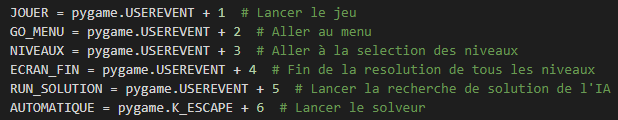
\includegraphics[scale=1]{images/Capture_093958.png}
	\captionof{figure}{Initialisation des évènements}
\end{center}

\subsection{La couche menu, la couche de sélection de niveau et la couche de fin}

Ces couches ont été développées principalement pour améliorer l'interactivité côté utilisateur. Ainsi du côté utilisateur, ces couches se présentent comme une
interface dans laquelle on peut défiler et sélectionner un bouton.
\begin{itemize}
	\item \textbf{La couche menu}: Sur cette couche, l'utilisateur a le choix entre démarrer une partie, aller à la sélection des niveaux ou quitter la partie. Côté programmation, nous effectuons principalement l'affichage graphique et postons des évènements.
	\\
	\\
	\item \textbf{La couche de sélection de niveau}: L'intérêt principal de cette couche est de présenter une liste de niveaux que l'utilisateur pourra sélectionner. Du point de vue programme, cette couche permet de récupérer le niveau sélectionné par l'utilisateur, gère le côté graphique et permet de poster l'évènement \textbf{JOUER} quand on sélectionne un niveau.
	\item \textbf{La couche de fin}: Cette couche apparaît quand l'utilisateur termine la résolution du niveau 10. Il affiche le nombre de coups Total et donne les options de poursuites du jeu.
\end{itemize}
\begin{figure}[!ht]
	\begin{subfigure}[b]{0.3\textwidth}
		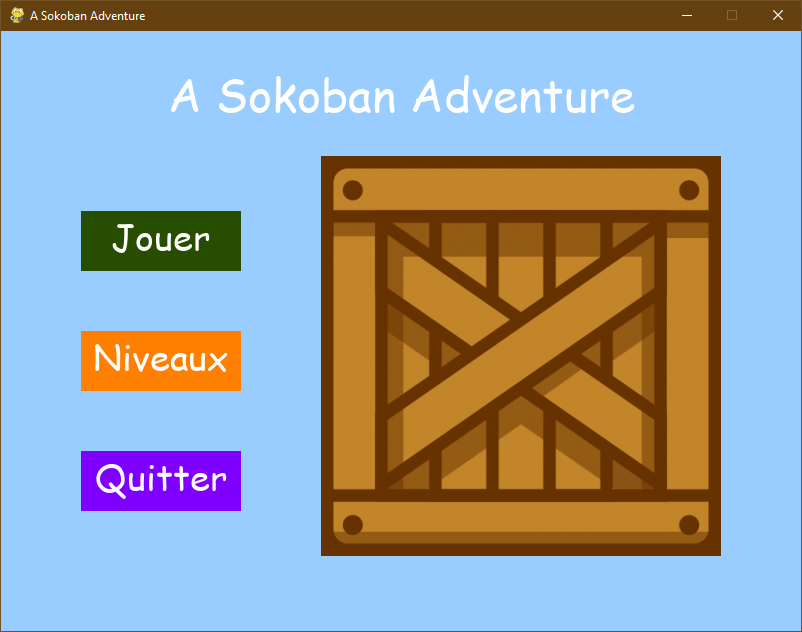
\includegraphics[width=\textwidth]{images/Capture_100726.png}
		\caption{La couche menu}
	\end{subfigure}
	\begin{subfigure}[b]{0.3\textwidth}
		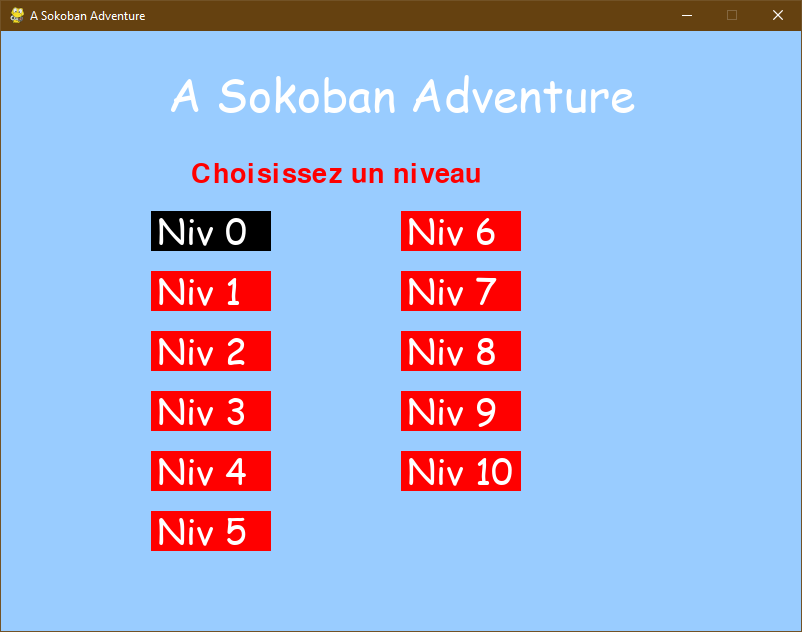
\includegraphics[width=\textwidth]{images/Capture_102044.png}
		\caption{La couche de sélection}
		\end{subfigure}
	\begin{subfigure}[b]{0.3\textwidth}
		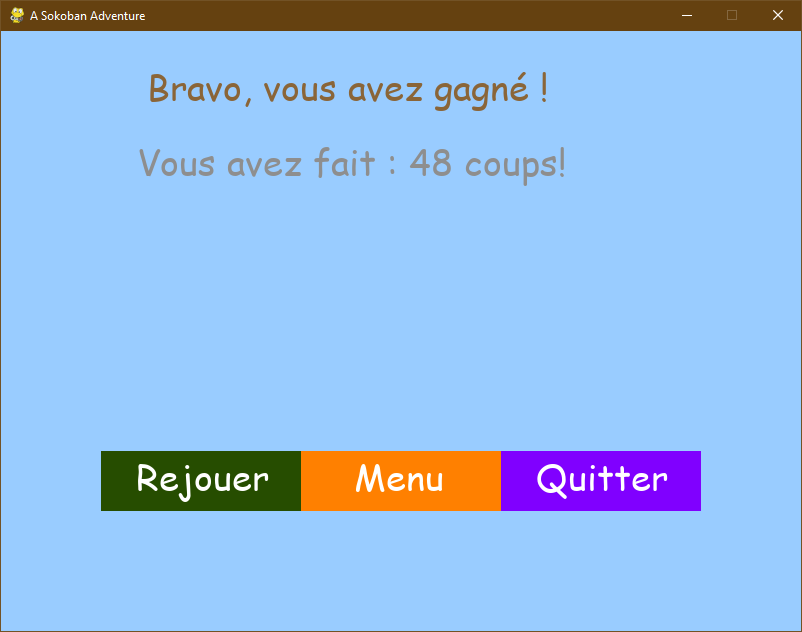
\includegraphics[width=\textwidth]{images/Capture_104740.png}
		\caption{La couche de fin}
	\end{subfigure}
	\caption{Les couches intermédiaires}
\end{figure}
	

\subsubsection{Les boutons} 

Les boutons ont été considérés comme des rectangles de couleurs sur lesquels on peut écrire du texte et modifier également la couleur en fonction de la présence de l'utilisateur sur ce dernier.
\newline
Ainsi pour chaque couche de jeu où il est nécessaire de faire apparaître des boutons sur l'écran, on procède par étape:

\begin{itemize}
	\item Définir la taille de chaque rectangle à travers  \textbf{pygame.Rect}.
	\item Associer chaque bouton à un rectangle mais aussi les dessiner et les positionner sur l’écran avec \textbf{pygame.draw.rect}.
	\item Définir le texte qui sera affiché sur le rectangle.
\end{itemize}
Sur un écran, on peut défiler entre les différents boutons grâce aux touches directionnelles. Actionner un bouton est possible grâce à un attribut des couches \textbf{bouton\_token}.
Cet attribut prend le numéro du bouton sur lequel on est actuellement positionné. Lors de leur activation, selon le bouton, un évènement précis est posté dans la file d'attente des évènements. C'est grâce à cela que l'on peut actionner la bonne fonctionnalité.
\begin{center}
	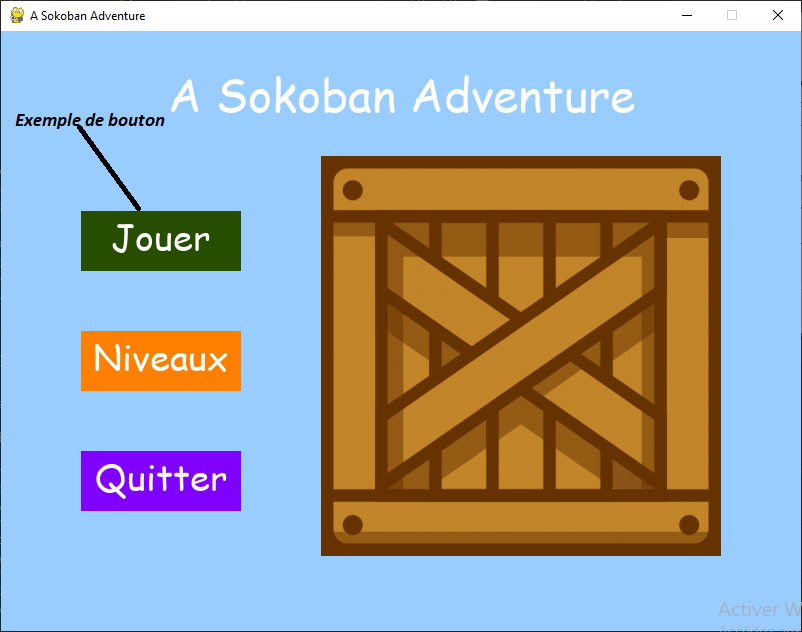
\includegraphics[scale=0.4]{images/Capture_133201.png}
	\captionof{figure}{Illustration d'une couche possédant des boutons}
\end{center}

\subsubsection{Le score} 

Le score a été considéré comme étant le nombre de niveau que l'utilisateur a résolu lors d'une partie de jeu. Ainsi, on peut l’incrémenter de 1 uniquement quand l'utilisateur a terminé la résolution d'un niveau. C'est une donnée qui est disponible uniquement quand l'utilisateur est dans une partie en cours (\textbf{couche de jeu}).

\subsection{La couche de jeu}

La couche de jeu est l'une des plus importantes car elle représente l'état lorsque l'utilisateur est en pleine partie. Sur l'implémentation, elle ne diffère pas des autres couches. Toutefois, elle possède des données supplémentaires et fait également appelle à d'autres objets déjà implémentés.

Cette couche représente le carrefour de l'ensemble du projet. En effet, elle fait appel à l'utilisation des objets importants déjà implémentés (\textbf{Level, Image}).
\\
Dès l'initialisation de la couche de jeu, on définit :

\begin{itemize}
	\item Le numéro du niveau: de 0 à 10
	\item On construit le niveau à partir de l'objet Level
	\item On charge les images de jeu sokoban avec l'objet Image
	\item On définit le score, le nombre de coup, le nombre de coups total
	\item On définit les touches de déplacement que l'on utilisera dans la partie.
\end{itemize}
C'est dans cette couche que l'on gère à proprement dit la résolution d'un niveau de la part de l'utilisateur.
\begin{center}
	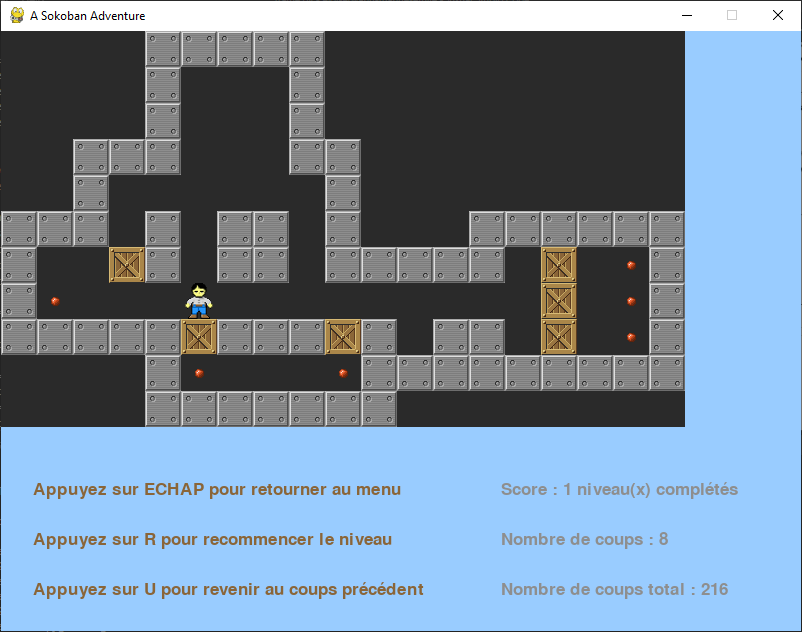
\includegraphics[scale=0.40]{images/Capture_104539.png}
	\captionof{figure}{Illustration de la couche de jeu}
\end{center}
\subsubsection{L'objet Image}
La classe Image est une classe qui nous permet de charger des images du jeu et de les associer à des caractères précis.
Elle possède deux(2) principales méthodes qui permettent de pouvoir afficher sur un écran les images associées à ces caractères.
\begin{itemize}
	\item \textbf{dessiner\_grille}: Elle permet une représentation graphique d'une tableau 2D grâce à un parcours par ligne et colonnes.
	\item \textbf{dessiner\_level}: C'est une méthode qui est d'avantage liée à la conception de notre projet car elle permet la représentation graphique d'un Objet Grille ou level grâce à un parcours par numéro de cases.
\end{itemize}
Les deux(2) fonctionnent selon un même algorithme.
\\
\textbf{\emph{Début de la méthode:
\\
\tabto{2em}itération sur les éléments du tableau 2D(par ligne et colonne ou par numéro de case):
\\
\tabto{3em} tester si le caractère est dans le dictionnaire des caractères prédéfinis
\\
\tabto{4em} afficher le caractère sur l'écran à des coordonnées calculées selon sa position dans le tableau
\\	
Fin de la méthode}}
\\
\begin{center}
	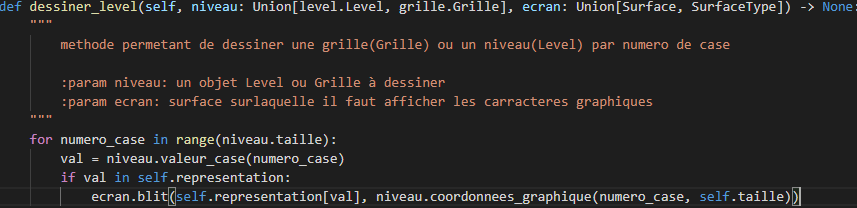
\includegraphics[scale=0.6]{images/Capture_121210.png}
	\captionof{figure}{Exemple pour la méthode \textbf{dessiner\_level}}
\end{center}

\newpage
\subsubsection{La méthode react\_to de la couche de jeu}

La méthode react\_to permet de récupérer les évènements claviers et de modifier ainsi certaines données. A travers les évènements récupérés, elle permet notamment le déplacement de l'utilisateur. Elle parvient à modifier les données à travers trois(3) éléments:

\begin{itemize}
	\item Les touches de jeu: Quand l'utilisateur utilise l'une des touches nécessaires aux déplacements du personnage, le nombre de coup et nombre de coup, le nombre de coups total sont incrémenter, le plateau de jeu (contruct) est modifié pour appliquer le déplacement.
	\item La touche résolution: Elle permet de basculer vers la couche de résolution qui permet de passer à la résolution du niveau courant.
	\item La victoire de l'utilisateur: On teste la condition de victoire, si elle est vraie alors on charge un nouveau niveau et on incrémente le score, ou alors on bascule sur la couche de fin.
\end{itemize}
\section{Les ajouts de confort de jeu}
Dans le but d'améliorer l'expérience de l'utilisateur, certaines fonctionnalités supplémentaires ont été pensées.

\subsection{Les indications textuelles}
Durant une partie, il semblait nécessaire d'ajouter certaines indications à l'utilisateur. Ces indications portent sur les informations que l'on recueille sur la partie en cours (score, nombre de coups, nombre de coups total....) mais aussi sur les touches qui permettent la navigation.
\begin{center}
	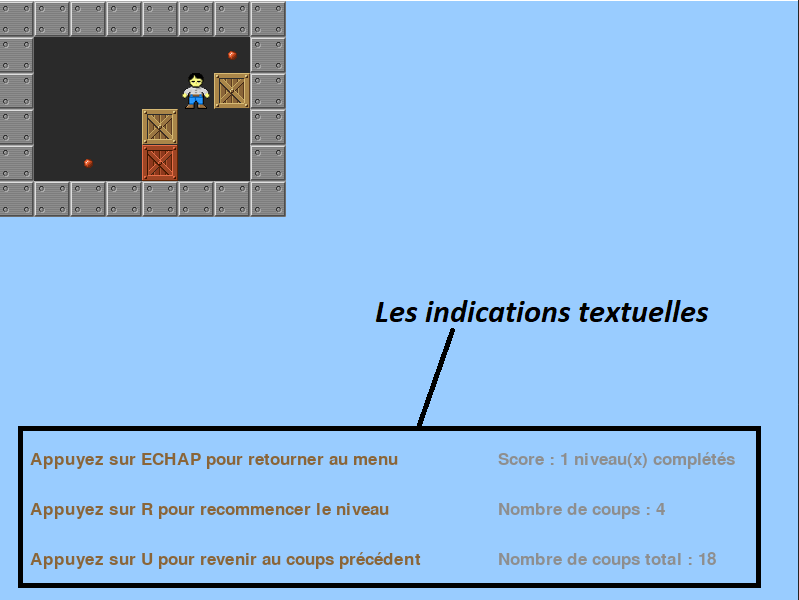
\includegraphics[scale=0.40]{images/Capture_102254.png}
	\captionof{figure}{illustrations d'un exemple d'indications textuelles}
\end{center}

\newpage
\subsection{Les sons du jeu}
Le son a été envisagé pour rendre le jeu moins banal, et ajouter une véritable sensation d'interaction du côté utilisateur.
Cela est réalisé dans le module multimédia qui contient un objet \textbf{Audio}, celui-ci charge l'ensemble des sons, et grâce à ces modules peut jouer l'un des sons.
Ainsi deux(2) principaux sons peuvent être écoutés par l'utilisateur:
\begin{itemize}
	\item Un son lorsqu'il appuie sur une touche du clavier.
	\item Un son pour le lancement d'une partie.
\end{itemize}

\subsection{Les touches de "sauvetage"}

Les touches de "sauvetage" sont des touches qui nous permettent de nous donner une seconde chance lors de la résolution d'un niveau. C'est à dire elles nous permettent d'effectuer soit un retour à la position précédente, ou tout simplement de recommencer le niveau au début.

\subsubsection{Le retour arrière}

Cette fonctionnalité s'avère pratique dans la mesure où l'utilisateur peut décider de modifier son déplacement.
Cela fait appel à la méthode \textbf{dernier\_plateau} de l'objet \textbf{Level}.
Cette méthode effectue un \textbf{pop} sur l'attribut \textbf{historique}\footnote{l'attribut historique de level est une liste python qui contient l'ensemble des plateaux } de \textbf{level} ce qui nous permet de remplacer le plateau courant par le dernier des plateaux tout en le supprimant de l'historique.
Ainsi durant une partie, l'utilisateur, en appuyant sur la touche "u", peut revenir au déplacement précédent.

\subsubsection{La remise à zéro du niveau}

A l'initialisation d'un niveau, une copie de son plateau est préalablement enregistrée ce qui permet de remettre tout à zéro sans pour autant faire une nouvelle initialisation de l'objet.


\section{L'algorithme de résolution}

\subsection{Recherche d'un algorithme compatible}

Au départ, nous souhaitions implémenter un algorithme écrit par nos soins, nous avons donc commencé à nous renseigner sur l'algorithme A*, cependant faute de temps, nous avons dû nous résoudre à trouver un algorithme compatible que nous pourrions adapter.

Pour cela nous nous sommes rendus sur \href{https://github.com/}{GitHub} et avons, dans un premier temps, cherché des solveurs de Sokoban codés en Python.

Une fois que nous en avions trouvé plusieurs, nous avons commencé à les tester. Lors de ces tests, un solveur a particulièrement retenu notre attention, car nous pouvions utiliser plusieurs algorithmes : le BFS (Breadth First Search, ou Algorithme de parcours en largeur), le DFS (Depth First Search, ou Algorithme de parcours en profondeur), l'UCS (Uniform Cost Search) et le A*. 

Ce solveur a été écrit par \textit{KnightofLuna}, et vous pouvez y accéder en cliquant sur  \href{https://github.com/KnightofLuna/sokoban-solver}{ce lien GitHub}.

Cependant, nous nous sommes heurtés à un problème : les temps de résolution des niveaux complexes par les différents algorithmes. Pour plus de détails, vous pouvez consulter l'annexe C \ref{algorithme}.

\subsection{Adaptation de l'algorithme}

\subsubsection{Modifications du programme}

Afin que le solveur puisse directement fonctionner avec nos fichiers .sok, nous avons dû effectuer une modification sur les caractères utilisés pour définir le personnage, les murs, les caisses, les emplacements de caisse, et les caisses sur un emplacement de caisse (qui sont respectivement @, \#, \$, ., *). De plus, nous avons dû ajouter la possibilité que le personnage soit sur un emplacement de caisse grâce au caractère +.
Nous avons également modifié les actions possibles afin que celles-ci puissent être directement utilisées dans notre solveur automatique, à savoir : 
\begin{itemize}
	\item un coup vers le haut est désormais représenté par un h si le joueur ne pousse aucune caisse, et par un H si le joueur déplace une caisse;
	\item un coup vers le bas est désormais représenté par un b si le joueur ne pousse aucune caisse, et par un B si le joueur déplace une caisse;
	\item un coup vers la gauche est désormais représenté par un g si le joueur ne pousse aucune caisse, et par un G si le joueur déplace une caisse;
	\item un coup vers la droite est désormais représenté par un d si le joueur ne pousse aucune caisse, et par un D si le joueur déplace une caisse.
\end{itemize}

Enfin, nous avons décidé de ne garder que l'algorithme A*, et donc de supprimer les algorithmes BFS, DFS, et UCS, car ceux-ci prennent trop de temps à résoudre les niveaux pour être utilisés dans notre solveur automatique.


\subsubsection{Intégration de l'algorithme au jeu}
L'algorithme a été intégré au jeu en implémentant une nouvelle couche. Cette couche ne diffère pas des autres du point de vue de l'implémentation.
En particulier, lors de l'initialisation, la recherche de solution par l'IA est lancée. Vu la complexité de certains niveaux, la recherche peut être longue.
De ce fait, nous avons choisi de limiter le temps de recherche à \textbf{5 secondes}. L'algorithme A* étant le plus pratique du point de vue du temps, pour certains niveaux, nous avons du faire en parallèle la recherche d'une solution par d'autres méthodes. Ainsi, pour l'ensemble des niveaux présents dans le fichier de base, nous sommes
à mesure de fournir une solution.

\newpage

\section{Manuel d'utilisation et Illustration de l'usage}
\subsection{Manuel d'utilisation}
\textbf{" A Sokoban Adventure"} est un jeu à l'interface graphique simple et compréhensible par l'utilisateur. Votre but principal est de terminer la résolution de chacun des niveaux. Pour terminer un niveau, vous avez besoin de placer l'ensemble des caisses sur les emplacements prédéfinis.
Au cours de vos parties, diverses fonctionnalités du jeu vous permettront de parvenir à ce but.\\
Ce jeu ne demande aucun prérequis particulier pour y jouer. 
\subsubsection*{a - Comment jouer?}
Pour jouer, vous auriez besoin d'un clavier alphanumérique. L'utilisation d'une souris n'est pas nécessaire.\\
Pour démarrer le jeu, il vous faudra lancer la lecture du fichier "main.py". Pour cela deux(2) possibilités s'offrent à vous :
\begin{itemize}
	\item Posséder un \textbf{IDLE}: Il vous faudra alors ouvrir le répertoire du jeu dans l'iddle et lancer la lecture du fichier \textbf{main.py}
	\item Lancement dans un \textbf{Terminal}: Dans le terminal vous devrez vous trouver dans le répertoire du jeu et lancer la commande \emph{\textbf{python main.py}}
\end{itemize}
Une fois lancer vous auriez la possibilité de lancer directement une partie ou de choisir le niveau que vous souhaiterez résoudre
\subsubsection*{b - Guide de commande}
\begin{table}[!ht]
	\begin{tabular}{|l|l|l|l|l|}
		\hline
		\multicolumn{2}{|l|}{\textbf{Touches}}                                                                                                                                         & \multicolumn{3}{l|}{\textbf{Utilisations}}                  \\ \hline
		\multicolumn{2}{|l|}{\Touche{ $\leftarrow$} \Touche{$\uparrow$} \Touche{$\rightarrow$} \Touche{$\downarrow$}} & \multicolumn{3}{l|}{Se déplacer entre les boutons} \\ \hline
		\multicolumn{2}{|l|}{\Touche{Space} / \Touche{$\hookleftarrow$} ou \Touche{Enter}}                                                                                                                                 & \multicolumn{3}{l|}{Valider}                       \\ \hline
		\multicolumn{2}{|l|}{\Touche{echap} ou \Touche{esc}}                                                                                                & \multicolumn{3}{l|}{Revenir au menu}               \\ \hline
		\multicolumn{2}{|l|}{\Touche{m}}                                                                                                                                     & \multicolumn{3}{l|}{Couper le son}                 \\ \hline
	\end{tabular}
	\caption{Les touches utilisables entre les écrans}
\end{table}

\begin{table}[!ht]
	\begin{tabular}{|l|l|l|l|l|}
		\hline
		\multicolumn{2}{|l|}{\textbf{Touches}}                                                                                                                                         & \multicolumn{3}{l|}{\textbf{Utilisations}}                  \\ \hline
		\multicolumn{2}{|l|}{\begin{tabular}[c]{@{}l@{}}\Touche{ $\leftarrow$} \Touche{$\uparrow$} \Touche{$\rightarrow$} \Touche{$\downarrow$} \\ ou \\ \Touche{Q} \Touche{Z} \Touche{D} \Touche{S} \end{tabular}} & \multicolumn{3}{l|}{Déplacer le personnage respectivement à gauche/ haut/ droite/ bas} \\ \hline
		\multicolumn{2}{|l|}{\Touche{R}}                                                                                                                                                                                                                                                                                                                                                                              & \multicolumn{3}{l|}{Réinitialiser le niveau en cours}                                  \\ \hline
		\multicolumn{2}{|l|}{\Touche{U}}                                                                                                                                                                                                                                                                                                                                                                              & \multicolumn{3}{l|}{Effectuer un undo (revenir à la position précédente)}               \\ \hline
		\multicolumn{2}{|l|}{\Touche{P}}                                                                                                                                                                                                                                                                                                                                                                              & \multicolumn{3}{l|}{Lancer la recherche de solutions (solver)}                           \\ \hline
		\multicolumn{2}{|l|}{\Touche{Space}}                                                                                                                                                                                                                                                                                                                                                                          & \multicolumn{3}{l|}{Démarrer la résolution automatique}                                 \\ \hline
		\multicolumn{2}{|l|}{\Touche{$\hookleftarrow$} ou \Touche{Enter}}                                                                                                                                                                                                                                                                                                                                           & \multicolumn{3}{l|}{Si vous êtes dans le solveur, revenir à l'écran de jeu}            \\ \hline
		\multicolumn{2}{|l|}{\Touche{echap} ou \Touche{esc}}                                                                                                                                                                                                                                                                                                                                                         & \multicolumn{3}{l|}{Revenir au menu}                                                   \\ \hline
		\multicolumn{2}{|l|}{\Touche{m}}                                                                                                                                                                                                                                                                                                                                                                              & \multicolumn{3}{l|}{Couper le son}                                                     \\ \hline
	\end{tabular}
	\caption{Les touches utilisables lors d'une partie}
\end{table}


\subsection{Illustration de l'usage}
\begin{center}
	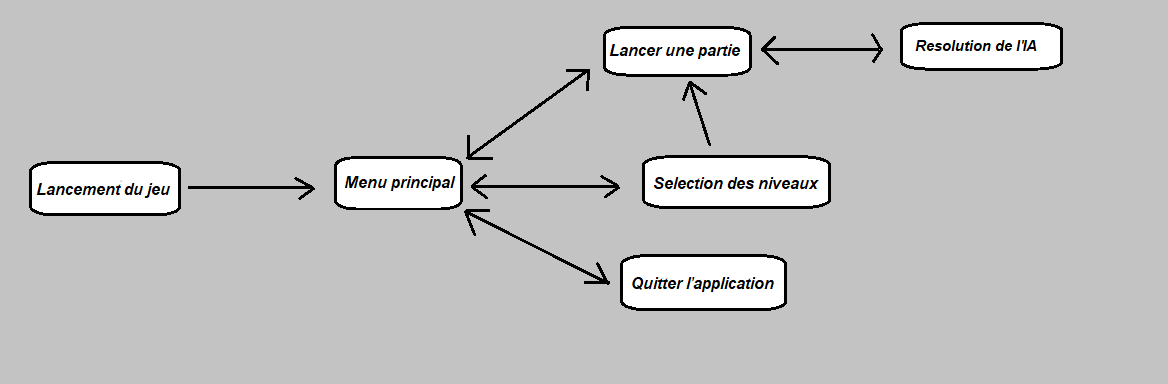
\includegraphics[scale=0.5]{images/Cas_d'utilisation.png}
	\captionof*{figure}{diagramme d'utilisation}
\end{center}
Ce diagramme résume l'ensemble de cas d'utilisation que l'on peut avoir quand l'utilisateur souhaiterait démarrer le jeu.
\newpage

\section{Possibles améliorations} 
Bien que le rendu du projet nous paraisse plus que complet, de par sa stabilité et ses nombreuses fonctions améliorant le confort de jeu, nous gardons à l'esprit qu'il reste  grandement améliorable car limité par notre période de développement et les limitations de nos compétences. Si nous devions revenir dessus avec plus de temps et de savoirs, nous avons pensé à quelques améliorations.
\begin{itemize}
\item Dans un premier temps, il serait intéressant de pouvoir intégrer des niveaux personnels au jeu simplement par l'intermédiaire d'une interface sur le logiciel qui permettrait à l'utilisateur de définir un chemin vers ce niveau sur l'ordinateur puis l'ajouter à la liste des niveaux. Un ajout de confort qui irait dans ce sens serait l'implémentation d'un nouveau bouton pour le niveau ajouté sur l'interface de sélection des niveaux du Menu.
\item Dans le même registre mais nécessitant un savoir bien plus poussé, un générateur de niveau ou une interface de création de niveaux serait aussi une possible amélioration du logiciel. Cela ajouterait de la variété au jeu tout en évitant à l'utilisateur de passer par un fichier .sok pour ajouter son niveau au jeu, rendant la visualisation des niveaux créés bien plus claire.
\item Un des problèmes que nous avons rencontré lors de l'implémentation de l'algorithme de résolution au jeu a été de savoir comment proposer une résolution de niveau efficace sans bloquer l'écran trop longtemps à l'utilisateur. Une amélioration envisageable serait de permettre à l'algorithme de tourner pendant que l'utilisateur joue afin qu'il puisse commencer sa résolution à partir de l'endroit où se trouve le joueur au lieu de se contenter de montrer comment réussir le niveau du départ.
\item Un système de sauvegarde des scores, de comparaison avec un highscore pourrait aussi être un élément de comparaison entre les utilisateurs à la manière d'une borne d'arcade. De même, pouvoir voir le temps de résolution d'un niveau et diverses statistiques de joueur comme le nombre de déplacement moyen et le temps de résolution moyen par niveau pourrait s'avérer être un ajout intelligent. 
\end{itemize}
Voici un petit échantillon des nombreuses améliorations possibles du projet. Il serait intéressant d'y revenir en fin de cursus pour voir comment nos nouvelles connaissances nous permettraient d'améliorer le projet de différentes façons et surtout d'observer si les améliorations auxquelles nous avions pensées sont réellement réalisables.

\section{Conclusion}

Grâce à ce projet, nous avons pu approfondir nos connaissances en Python, notamment nos connaissances sur Pygame, mais également nos connaissances en algorithmie / algorithmique. De plus, nous avons pu découvrir le travail en équipe sur un projet d'assez longue durée, ce qui nous a permis de nous répartir le travail, en nous rapprochant du mode de fonctionnement que l'on peut trouver dans les entreprises.


\newpage
\section{Annexes}

\subsection*{A - Fichier .sok}

\begin{center}
	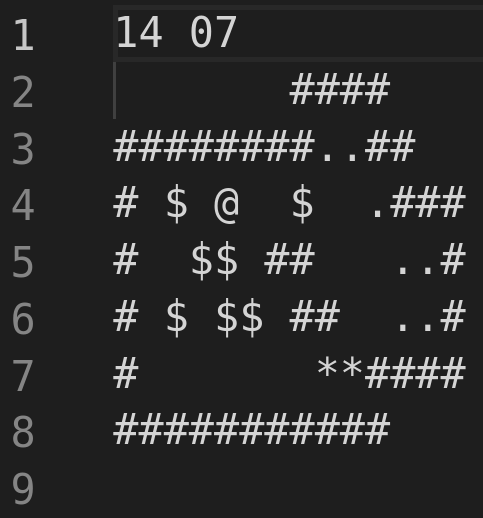
\includegraphics[scale=0.40]{images/Capture_212000.png}
	\captionof{figure}{Exemple de contenu d'un fichier .sok}
\end{center}

\subsection*{B - Les sources des fichiers multimedia}
\begin{itemize}
	\item Les images ont été récupérées du projet Sokoban, réalisé par \emph{Kazantzakis}, déposé sur ce lien \href{https://github.com/kazantzakis/pySokoban}{\textbf{\emph{GitHub}}.}
	\item Les sons ont été téléchargés sur \href{https://freesound.org/}{\textbf{\emph{freesound}}.}
\end{itemize}
\subsection*{C - Les différents algorithmes}
\label{algorithme}
Une absence de donnée (valeur égale à 0) signifie que nous n'avons pas pu exécuter l'algorithme jusqu'à ce qu'une solution soit trouvée car cela prenait beaucoup trop de temps et / ou beaucoup trop de mémoire vive (RAM).

\begin{center}
	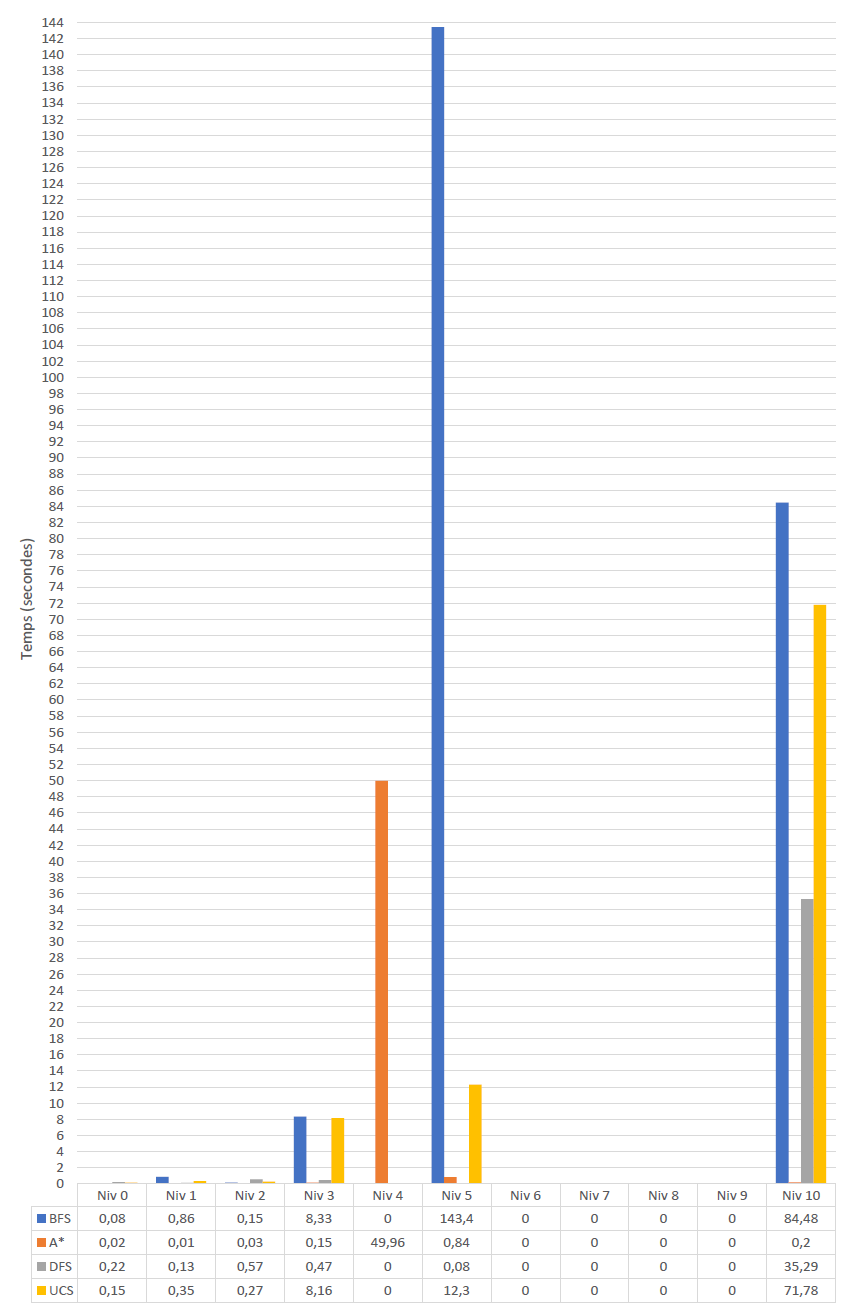
\includegraphics[scale=0.50]{images/Capture_143129.png}
	\captionof{figure}{Temps de résolution des niveaux en fonction des algortithmes utilisés}
	
	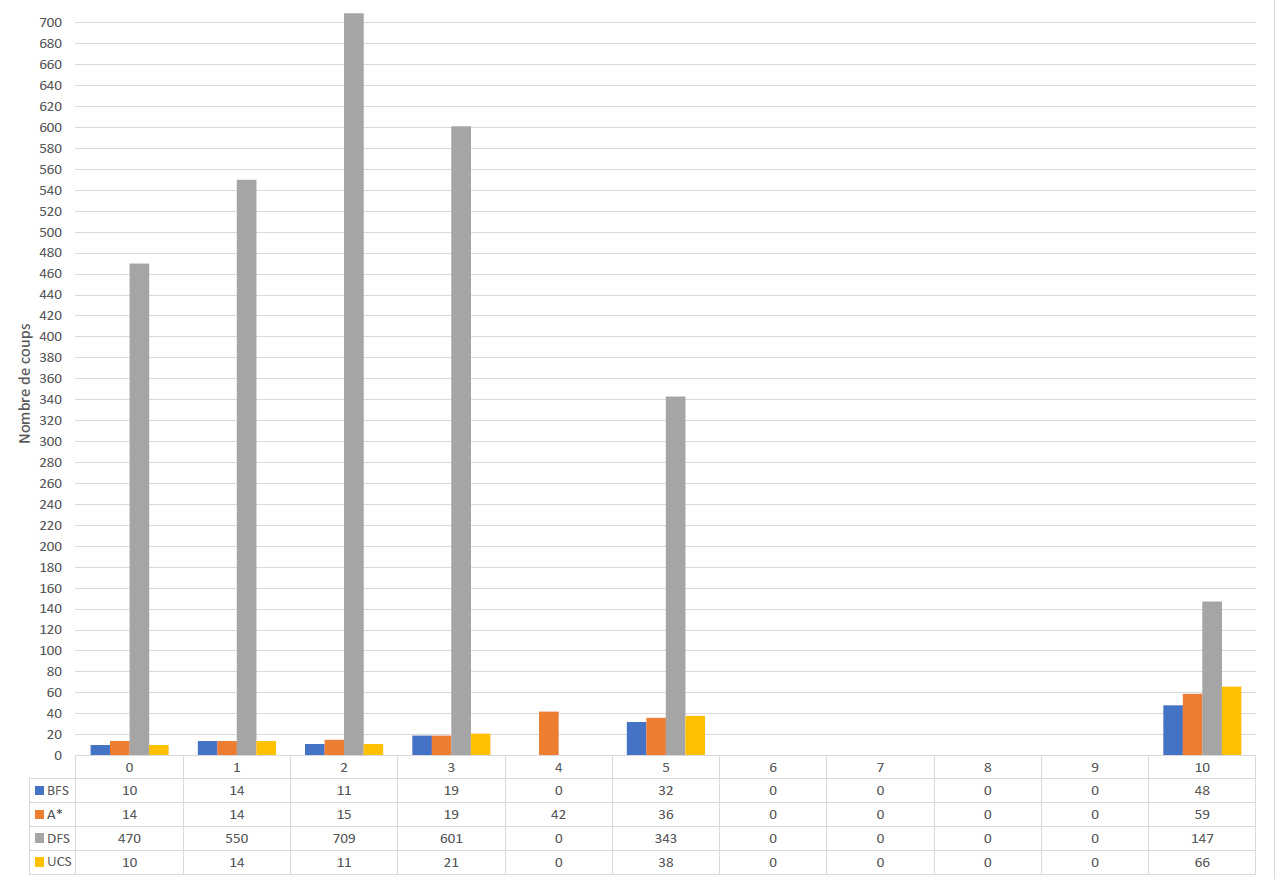
\includegraphics[scale=0.50]{images/Capture_143140.png}
	\captionof{figure}{Nombres de coups proposés pour résoudre les niveaux en fonction des algorithmes utilisés}
\end{center}

\subsection*{D - Les diagrames}
\subsubsection*{a - Diagramme de classe Grille}
\label{Grille}
\begin{center}
	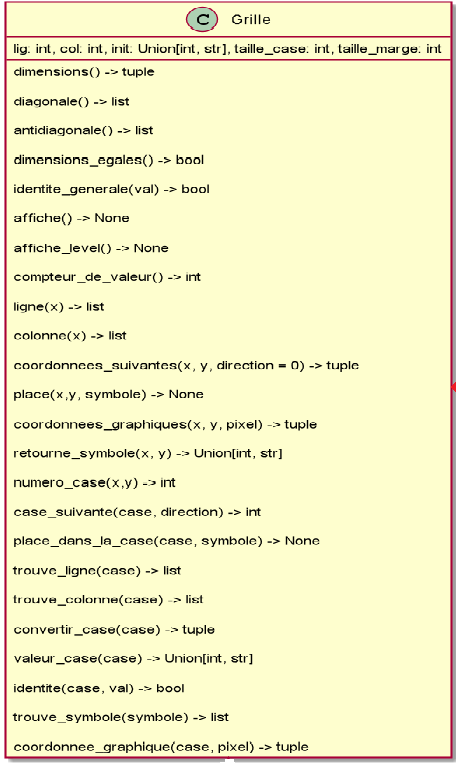
\includegraphics[scale=0.5]{images/classe_grille.png}
	\captionof{figure}{Diagramme de classe Grille}
\end{center}

\subsubsection*{b - Diagramme de classe Level}
\label{Level}
\begin{center}
	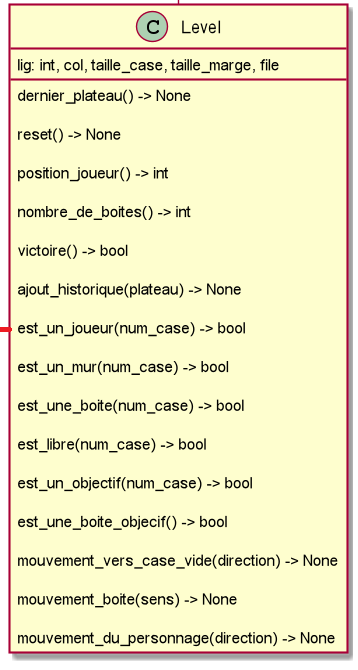
\includegraphics[scale=0.5]{images/classe_level.png}
	\captionof*{figure}{Diagramme de classe Level}
\end{center}

\subsubsection*{c - Diagramme Image et audio}
\label{multimedia}
\begin{center}
	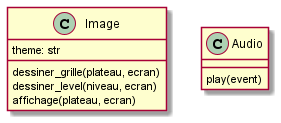
\includegraphics[scale=1]{images/multimedia.png}
	\captionof{figure}{Diagramme de Image et Audio}
\end{center}

\subsubsection*{d - Diagramme couches}
\label{couche}
\begin{center}
	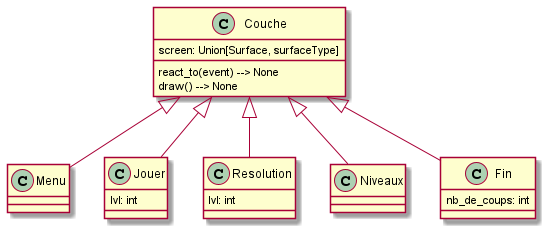
\includegraphics[scale=0.6]{images/frame.png}
	\captionof{figure}{Diagrammes des différentes couches}
\end{center}
\subsection*{E - Sources}
Voici la liste des sites consultés dans le cadre de la réalisation de notre projet :
\begin{itemize}
\item https://github.com/kazantzakis/pySokoban - GitHub - 23/10/2017 - kazantzkis
\\ Il s'agit du GitHub de la personne qui à developpé l'algorithme que nous avons adapté à notre projet.

\item https://fr.wikipedia.org/wiki/Sokoban - Wikipédia - 08/03/2021
\\ Page wikipédia décrivant les principes du Sokoban.

\item http://www.sokobano.de/wiki/index.php?title=Main\char`_Page - 23/06/2018
\\ Wikipédia/Encyclopédie dédié au Sokoban réunissant de nombreuses informations sur le jeu et ses différentes possibilités.

\item https://fr.wikipedia.org/wiki/Algorithme\char`_A* - Wikipédia - 23/03/2021
\\ Page wikipédia décrivant les principes de l'algorithme de résolution A*.

\item https://fr.wikipedia.org/wiki/Algorithme\char`_anytime - Wikipédia - 28/09/2017
\\ Page wikipédia décrivant le principe d'un algorithme anytime en informatique.

\end{itemize}

\end{document}